\documentclass[a4,12pt]{scrartcl}

%Basic 
\usepackage[utf8]{inputenc}
\usepackage[ngerman]{babel}
\usepackage[T1]{fontenc}
\usepackage{float}
\usepackage[bottom = 3.50cm]{geometry}

%Titel Seite
\title{CLOUD INFRASTRUCTURE}
\subtitle{Lab-07}
\author{Giorgio Vincenti \and Samuel Krieg}
\date{\today}


%Kopf, Fusszeile
\usepackage{fancyhdr}
\pagestyle{fancy}
\lhead{ \begin{picture}(0,0) \put(0,0){
\includegraphics[width=3cm]{./pictures/hsrlogo.png}} \end{picture}}
\chead{}
\rhead{Seite \thepage}
\lfoot{Cloud Infrastructure \\Lab-07}
\cfoot{Giorgio Vincenti \and Samuel Krieg}
\rfoot{\today}
\renewcommand{\headrulewidth}{0.4pt}

%Bilder
\usepackage{graphicx}

%Tabellen
\usepackage{booktabs}

%Codesnippets
\usepackage{listings}
\lstset{language=bash} 

%Querformat für eine Seite
\usepackage{lscape}
\usepackage{rotating}
\usepackage{pdflscape}

%Temp
\usepackage{lipsum}



\begin{document}

\clearpage\maketitle
\thispagestyle{empty}
\tableofcontents
\newpage

\section{Research modern data center requirements}
\subsection{Challenges}
\begin{itemize}
\item new traffic behavior
\item management of computing nodes
\item higher security risks
\item new staff required
\end{itemize}

\subsection{Requirements}
\begin{itemize}
\item Elastic Auto-Scaling
\item Mobility of Applications, Systems and Data
\item Multi-Tenancy
\item Highest Availability
\item Autoprovisioning of Applications, Systems and Data
\end{itemize}

\subsection{Network architecture}
\begin{itemize}
\item Scalability
\item Managing higher traffic in DC
\item capable of "Elephant flows"
\end{itemize}

\section{TRILL}
\textbf{Tr}ansparent \textbf{I}nterconnection of \textbf{L}ots of \textbf{L}inks ist ein von der IETF festgelegten Standard.
\subsection{Funktion / Protokoll-Header}
\subsubsection{Funktion}
TRILL ist eine kombination von Layer 2 und Layer 3. Es ermöglicht auf Layer 2 zu routen und ersetzt Spanning Tree Protocol.
\subsubsection{Header}
\begin{figure} [H]
	\begin{center}
	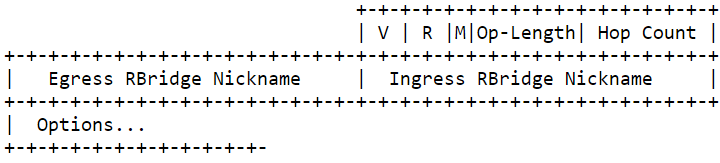
\includegraphics[width=0.80\textwidth]{./pictures/trill_header.png}
	\caption{\textbf{TRILL Header}}
	\label{x}
	\end{center}
\end{figure}
\begin{itemize}
\item V (Version): 2-bit unsigned integer.
\item R (Reserved): 2 bits.
\item R (Reserved): 2 bits.
\item Op-Length (Options Length): 5-bit unsigned integer.
\item Hop Count: 6-bit unsigned integer.
\item Egress RBridge Nickname: 16-bit identifier.
\item Ingress RBridge Nickname: 16-bit identifier.
\item Options: present if Op-Length is non-zero.
\end{itemize}

\subsection{Goal of TRILL:}
To uses Layer 3 routing techniques to create a large cloud of links which appear to IP nodes to be a single IP subnet. 

\subsection{Why was TRILL developed?}
\textbf{Tr}ansparent \textbf{I}nterconnection of \textbf{L}ots of \textbf{L}inks TRILL allows the ease of configuration of Ethernet while benefitting from the routing techniques provided at Layer 3.

\subsection{Where and how can TRILL be used?}
In datacenter for better migration of virtual machines. There will also be more bandwidth available for intensive applications like real-time communications and for the transport of storage traffic across the Ethernet network with FCoE and iSCSI.

\subsection{Is TRILL comparable to a traditional protocol?}It's a combination of traditional protocols (Ethernet, IP) and it's a bit like MPLS.
\subsection{What are the advantages and disadvantages of TRILL?}
TRILL make switches more cost-effective because it allows to load balance and to use more links in data center network designs.
Reduces Latency and improves overall network bandwidth utilization.
\subsection{Are there other modern technologies which are similar to TRILL} multichassis link aggregation or shortest path bridging
\subsection{How is TRILL configured in the LAB?}
\subsubsection{Trees}
\subsubsection{PacketFlow}
\subsubsection{MAC Learning}
\section{VXLAN}
\section{VXLAN with Arista switches}
\section{VXLAN Configuration}
\section{Research modern data center requirements}
Text


\subsection{Subsection}
Text


\subsubsection{Subsubsection}
Text

\section{Aufzählung}
\subsection{Itemize}
\begin{itemize}
\item Das erste Item
\item Das zweite Item
\begin{itemize}
\item Das erste Item
\item Das zweite Item
\item Das dritte Item
\end{itemize}
\item Das dritte Item
\end{itemize}

\subsection{Enumerate}
\begin{enumerate}
  \item The first item
  \item The second item
  \item The third etc \ldots
\end{enumerate}

\subsection{Description}
\begin{description}
  \item[First] The first item
  \item[Second] The second item
  \item[Third] The third etc \ldots
\end{description}
\begin{description}
  \item[First] \hfill \\
  The first item
  \item[Second] \hfill \\
  The second item
  \item[Third] \hfill \\
  The third etc \ldots
\end{description}

\section{Tabellen}
\begin{center}
    \begin{tabular}{@{} l l r@{}}\toprule    
    {Stockwerk} & {Hostname} & {Anzahl Ports}\\ \midrule
    1 & DataCSW01 & 12\\ \addlinespace
    & DataCSW03 & 12\\ \addlinespace
    & DataCSW04 & 12\\ \addlinespace
    2& DataCSW02 & 24\\
    \bottomrule
    \end{tabular}
\end{center}

\section{Codesnippets}
\begin{lstlisting}
sudo apt-get install qemu
\end{lstlisting}

\section{Bilder}
\begin{figure} [H]
	\begin{center}
	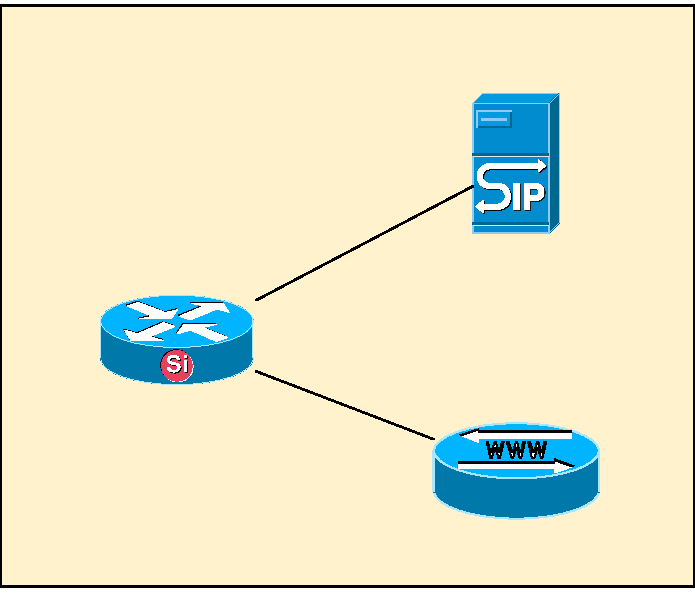
\includegraphics[width=0.50\textwidth]{./pictures/sample_picture.pdf}
	\caption{\textbf{Bild Unterschrift}}
	\label{Bild Referenz}
	\end{center}
\end{figure}

\begin{landscape}
\begin{figure}[htbp]
\subsection{Querformat}
\centering
\fbox{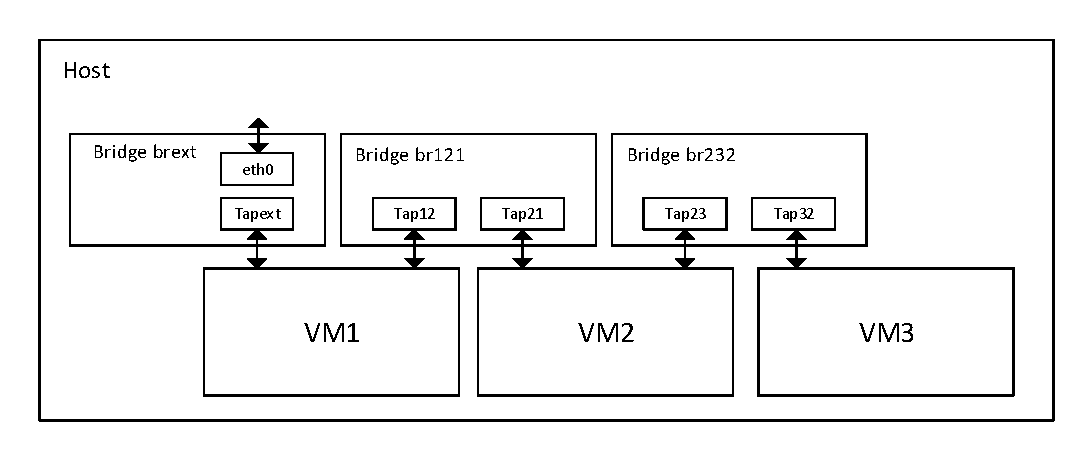
\includegraphics[width=\linewidth, height=\textheight,keepaspectratio]{./pictures/sample_picture_landscape.pdf}}
\caption{\textbf{Bild Querformat}}
\end{figure}
\end{landscape}	


\end{document}
